\documentclass{beamer}
\usepackage[utf8]{inputenc}
\usepackage[]{hyperref}
\usepackage{booktabs}
\usetheme[pageofpages=of,bullet=square,
	titleline=true,
	alternativetitlepage=true,
	titlepagelogo=figs-slides/distribs00.pdf]{Torino}

\author{Statistical Reasoning\\and Quantitative Methods}
\title{Distributions}
\institute{François Briatte \& Ivaylo Petev}
\date{Session 4}

\include{beameradditions}

\begin{document}
		
	\begin{frame}[t,plain]
		\titlepage
	\end{frame}
	
	\begin{frame}[t]{Launch your research project!}
	
		Fill in the details at \rd{\url{http://goo.gl/brYmB}}\\[1em]
		
		\includegraphics[width=.6\textwidth]{figs-slides/wordle-srqm-2012-1.pdf}
	
		\begin{itemize}
			\item Form a pair in your own group.
			\item Write up a clear title.
		\end{itemize}
	
		If you want to make any background reading on your topic, now is the right time to do so. Download and start editing the paper template at \rd{\url{http://goo.gl/7u8oa}} if you need a writing guide.

	\end{frame}
	
	\begin{frame}[t]{Outline}
	
	\red{Univariate statistics} look at the distribution of one variable and are part of \red{descriptive statistics}.
	
		\begin{columns}[T]
		\column{.35\textwidth}
			\tableofcontents[hideallsubsections]
		\column{.6\textwidth}
			\begin{center}
				\includegraphics[scale=.4]{figs-slides/distribs0.pdf}
			\end{center}		
		\end{columns}
	\end{frame}
	

	\section{Central tendency}

	\subsection{Mean}
	
	\begin{frame}[t]{Mean}

	\textbf{The \red{arithmetic mean}} $\bar X$ (or ``x bar'') of variable $X$ with $N$ observations is given by the following formula:
	
	$$\red{\bar{X}} = \frac{\displaystyle X_1+X_2+...+X_N}{\displaystyle N} = \red{\frac{1}{N}\sum_{i=1}^N X_i}$$

	\begin{itemize}
		\item Mean values can be calculated in several ways, but arithmetic means (\red{averages}) are by far the most common.
		
		\item Mean values are not robust to extreme values: their values are very \red{sensitive to outlier observations}.
				
		\item If $X_1, X_2,... , X_N$ are all weighted by a coefficient $w_i$, the arithmetic \red{weighted mean} is given by $\sum_{i=1}^N w_i \cdot X_i$, with $\sum_{i=1}^N w_i = 1$.
	\end{itemize}

	\end{frame}
	
	\begin{frame}[t]{Example: GDP/capita}

	Using country-level real GDP/capita, measured by the \href{http://unstats.un.org/unsd/snaama/}{United Nations Statistics Divisions -- National Accounts} in 2009:
	
	$$\textsf{Real GDP/capita} = \frac{\textsf{Real GDP}}{\textsf{population}} = \frac{\textsf{GDP}}{\textsf{population}} \cdot \textsf{price index}$$

	\begin{itemize}
		\item The mean can \red{summarise the distribution} of real GDP/capita in the full sample ($N = 192$) and/or in each geographical region.
		
		\item Average real GDP/capita will be \red{sensitive to exceptionally high or low values}, as with Somalia, Liechtenstein or Switzerland.
				
		\item Population and price act like \red{country-level weights}: all values of GDP are weighted by $\frac{\textsf{price index}}{\textsf{population}}$ to make them comparable.
	\end{itemize}

		On relative pricing, see Feinstein and Thomas, Appendix B.
	\end{frame}

	\fullslide{figs-slides/gdpc1.pdf}
	\fullslide{figs-slides/gdpc3.pdf}
	\fullslide{figs-slides/gdpc2.pdf}

	\subsection{Median}
	
	\begin{frame}[t]{Median}

	\textbf{The median value} is the \red{``middle'' of the distribution}:

	\begin{itemize}
		\item 50\% of the values fall below the median.
		\item 50\% of the values fall above the median.
	\end{itemize}

	\textbf{Unlike the mean}, it is \red{robust to extreme values}:
	
	\begin{columns}[t]
	\column{.7\textwidth}\vspace{-1em}
	\begin{itemize}
		\item Population: young Westerners, sample: class.
		\item Estimate values for mean and median income.
		\item Enter Facebook CEO. Recalculate estimates.
		\item Which value has just become very misleading?
	\end{itemize}
	\vspace{1em}
	\textbf{In your work}, adjust your reported measures of central tendency and select among graph types after looking at \red{both values} for the variable.
	\column{.25\textwidth}
	\begin{center}\vspace{-2.25em}
	\fbox{\includegraphics[scale=.1675]{figs-slides/zuckerberg.jpg}}
	\end{center}
	\end{columns}
	
	\end{frame}
	
	\subsection{Problem: median vs. mean}
	
	\begin{frame}[t]{Problem: median vs. mean}

		\begin{columns}[T]
			\column{.75\textwidth}
		\href{http://www.phdcomics.com/comics/archive.php?comicid=1086}{\includegraphics[height=.8\textheight]{figs-slides/phdcomics-salaries.jpg}}
	
				\column{.25\textwidth}
	True!\\
	\vspace{1em}
	Shockingly true!\\
	\vspace{1em}
	Yet:\\
	\vspace{1em}
		\href{http://junkcharts.typepad.com/junk_charts/2008/11/a-joke.html}{``What's the \red{median} salary of these football coaches?''}\\
	\vspace{1em}
	Result:\\
	\vspace{1em}
	\href{http://junkcharts.typepad.com/junk_charts/2008/11/a-joke.html}{Junk charts}.
		\end{columns}
	\end{frame}

	\subsection{Solution: Skewness}

	\begin{frame}[t]{Solution: \red{skewness}}

	Skewness measures the \red{symmetry of the distribution} by looking at the relative positions of the median and the mean:

	\begin{itemize}
		\item If $\textsf{median} > \textsf{mean}$, the distribution comes with a ``longer left tail'' and shows \red{``right-side skewness''}.
		\item If $\textsf{median} < \textsf{mean}$, the distribution comes with a ``longer right tail'' and shows \red{``left-side skewness''}.
	\end{itemize}
	
	\end{frame}
	
	\fullslide{figs-slides/hist1.pdf}
	\fullslide{figs-slides/hist2.pdf}

	\subsection{Mode}

	\begin{frame}[t]{Mode}
	\begin{columns}[T]
	\column{.35\textwidth}
	The mode is the `peak' of the distribution at its \red{most frequent value}.\\[1em]
	
	\red{Histograms} show the density of a distribution, to observe the mode and skewness.
	\column{.6\textwidth}
	\includegraphics[scale=.45]{figs-slides/hist3-white.pdf}
	\end{columns}

	\end{frame}

	\subsection{Stata: -su-, -tab-, -hist-…}
	
	\begin{frame}[t]{Stata: \code{su}, \code{tab}, \code{hist} etc.}
		
	\begin{itemize}
	\item \textbf{Formal} exploration:
	\begin{itemize}
		\item \code{su} (\code{summarize}) provides a \red{five-number summary} for the distribution of \red{continuous variables}.
		\item \code{tabstat} and \code{su} (\code{summarize}) with the \code{d} (\code{detail}) option provide percentiles and call the median \code{p50} or \code{50\%}, for ``\red{50\textsuperscript{th} percentile}.''
		\item \code{su} (\code{summarize}) with the \code{d} (\code{detail}) option also provides skewness, between --1 and +1, with \red{0 indicating symmetry}.
		\item \code{tab} or \code{fre} provide frequency tables with (cumulative and valid) percentages for \red{categorical variables}, to which only the mode applies.
	\end{itemize}
	
	\item \textbf{Visual} exploration:
	\begin{itemize}
		\item \code{hist} (\code{histogram}) shows the density of the distribution.
		\item \code{percent} and \code{addl} optionally add percentage scale and labels.
		\item \code{gr dot} is the most useful plot to visualize across categorical variables.
	\end{itemize}
	\end{itemize}
	
	% Concentrate on the \textbf{univariate statistics} with continuous variables. Categorical ones are used in comparisons, i.e. \textbf{bivariate statistics}.
	\end{frame}

	\begin{frame}[t]{Stata implementation}
	
	\begin{columns}
	\column{.35\textwidth}
	\begin{itemize}
	\item Explore the data with \code{lookfor} and \code{d}.
	\item Use \code{su} to summarise all variables at once.
	\item Use \code{su} with \code{d} on the dependent variable.
	\item Export a table with a \code{tabstat} sequence.
	\end{itemize}
	\column{.6\textwidth}	
	\begin{center}
		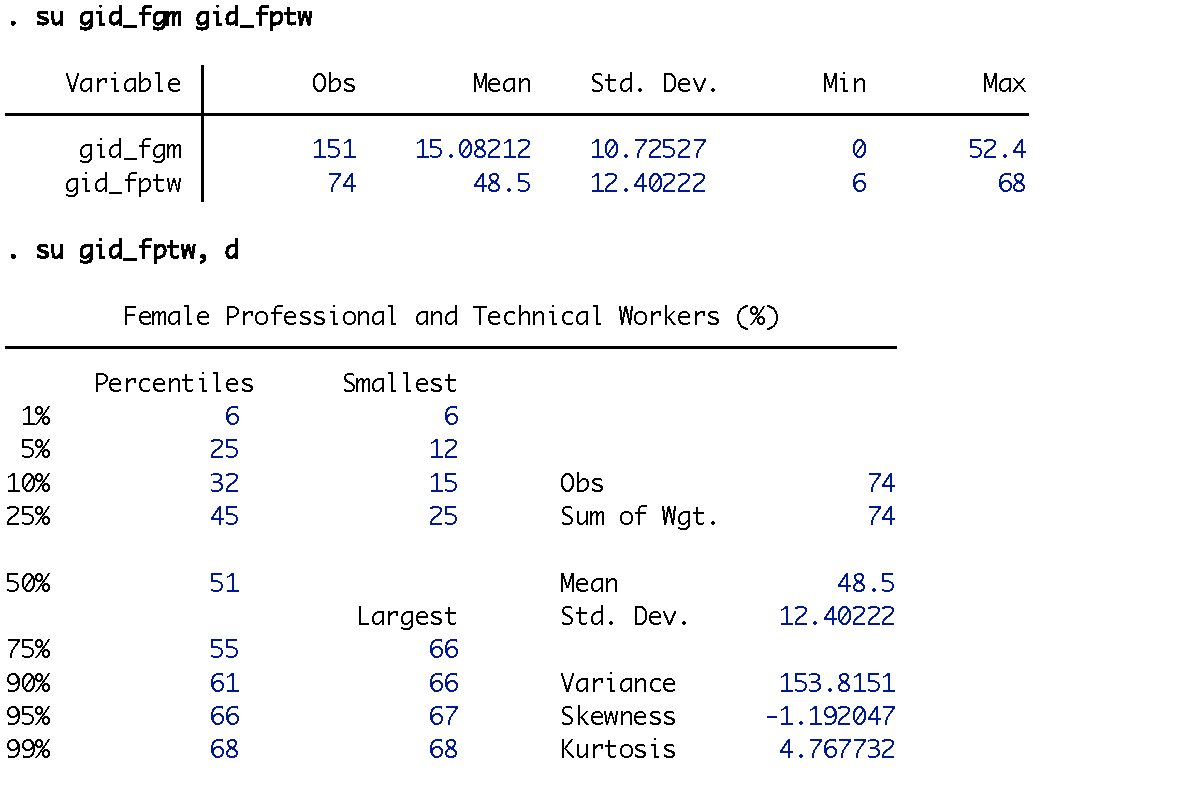
\includegraphics[scale=.3]{figs-slides/su.pdf}	
	\end{center}
	\end{columns}
	\vspace{1.5em}	
	Some descriptive measures will appear in the ``\red{summary statistics}'' table of your research, produced with a \code{tabstat} command sequence documented in the Stata Guide, Section 9.
	\end{frame}
	
	% \fullslide{figs-slides/hist3.pdf}
	% \fullslide{figs-slides/hist4.pdf}
	% [TR] ... this introduces VARIABILITY around the
	% measure of central tendency (mean/median/mode).
	
	%
	%
	%	
	\section{Variability}

	%
	%

	\subsection{Measures}

	% WRITE UP

	\begin{frame}[t]{Variability}

	\begin{itemize}
		\item \textbf{Range} is the `spread' of the variable $X$ between its maximum and minimum values: 
		
		\vspace{-1em}
		$$X_{max} - X_{min}$$
		
		\item \textbf{Variance} is the sum of \red{deviations from the mean}, $X_i - \bar X$, for each value taken by the variable $X$:
		
		\vspace{-1em}
		$$\sigma^2 = \sum_{i=1}^N (\red{X_i - \bar X})^2$$
		
		\item \textbf{Standard deviation} is the compound square root of variance divided by \red{sample size} $N$:

		\vspace{-1em}
		$$\sigma = \sqrt{\red{\frac{1}{N}} \sum_{i=1}^N (X_i - \bar X)^2}$$
	\end{itemize}
	
	\end{frame}

	\subsection{Quantiles}
	
	\begin{frame}[t]{Quantiles}

	% Example: income inequality
	
	Consider \textbf{income inequality} in \textbf{China} and the \textbf{United States}:
	
	\begin{quote}``Over the last 30 years, \red{top income shares} have increased substantially in English speaking countries and in India and China but not in continental Europe countries or Japan.''\\[.2em]-- Tony Atkinson, Thomas Piketty and Emmanuel Saez,\\ ``\href{http://piketty.pse.ens.fr/fichiers/public/AtkinsonPikettySaez2010.pdf}{Top Incomes in the Long Run of History},'' 2010.\end{quote}
		
	\begin{quote}``\red{1 percent of the people} take nearly a quarter of [U.S.] income.''\\[.2em]-- Joseph Stiglitz, ``\href{http://www.vanityfair.com/society/features/2011/05/top-one-percent-201105}{Of the 1\%, by the 1\%, for the 1\%},'' 2011.\end{quote}
	
	\begin{itemize}
		\item The ``top $p$\%'' principle uses \red{percentiles} to divide a distribution in 100 groups P1--P100 containing each 1\% of its values.
		\item Common divisions are \red{quartiles} (Q1--Q4) containing each 25\% of values, and \red{deciles} (D1--D10) containing each 10\% of values.
	\end{itemize}

	\end{frame}
	
	% the median democ. has just as many fem. minist. 
	% than the median dict.
	
	% fem. workers in democs are quasi-normal, bar Turkey and Bangl.
	% even the 25% democs with lowest fem. workers have more of them 
	% than half of dictatorships.

	\fullslide{figs-slides/income-top1percent.pdf}
	
	\subsection{Quartiles}

	\begin{frame}[t]{Quartiles, medians and box plots}

	\red{Histograms} are useful to compare a distribution with the normal distribution. \red{Box plots} have other purposes:

	\begin{itemize}
		\item \textbf{Detect outliers}, i.e. extreme observations: 
		
		\begin{itemize}
		
			\item Extreme observations \red{distort the mean}.
		
			e.g. Effect of Scandinavian countries on average female ministerial representation in democracies vs. dictatorships.
			
			\item Extreme observations	\red{reduce normality}.

			e.g. Effect of Turkey and especially Bangladesh on average and distribution of female worker rates in democracies.
		
		\end{itemize}
		
		\item \textbf{Compare groups}, i.e. over categories:
		
			\begin{itemize}
				\item With \red{binary} variables, e.g. male/female, democratic/dictatorial.
				
				\item With \red{nominal} variables, e.g. religion, ethnicity, geography.
				
				\item With \red{interval} variables, e.g. income groups, education levels.
			\end{itemize}
	\end{itemize}

	\end{frame}


	\begin{frame}[t]{Quartiles, medians and box plots}

	Box plot construction rules vary, but always show the \red{median} and \red{50\% of the distribution} as a `box' with `whiskers' at Q1 and Q3:
	
	\begin{center}
		\includegraphics[scale=.75]{figs-slides/boxplot-anatomy.pdf}	
	\end{center}

	\end{frame}

	\subsection{Stata: -gr box-}
	
	\begin{frame}[t]{Stata: \code{gr box}}
				
	\begin{columns}[T]
		\column{.7\textwidth}

		Box plot for worldwide female worker rates:\\

	\code{gr box workers, mark(1, mlabel(ccode))}\\[1em]

			\begin{itemize}
			\item \code{gr box} produces vertical box plots, \code{gr hbox} produces horizontal ones. Select the best.
			\item \code{mark(1, mlabel(ccode))} labels outliers with the variable \code{ccode} (country codes here).
			\item To compare one or more variables across groups, use either \code{over} or \code{by}.
		\end{itemize}
		More examples appear in the course do-files and in the Stata Guide, Section 9.
		\column{.25\textwidth}
		\includegraphics[height=.66\textheight]{figs-slides/boxplot-vertical.pdf}		
	\end{columns}
		
	\end{frame}
	
	%
	% NORMAL
	%
	
	\section{Normal distribution}

	\subsection{Distributions}
	
	\begin{frame}[t]{Distributions}
	
	\begin{itemize}
		\item \textbf{$\mu$} stands for the \red{mean} (central tendency).
		\item \textbf{$\sigma^2$} stands for \red{variance}, $\sigma$ for the \red{standard deviation} (variability).
	\end{itemize}
	
%	\includegraphics[width=\textwidth]{figs-slides/distributions.pdf}
%	\vspace{-1em}
%	\begin{columns}[t]
%		\column{.33\textwidth}
%			\begin{center}
%			% wvs_e069_14
%			Confidence in environmentalists\\[.5em]
%			\includegraphics[width=\textwidth]{figs-slides/distribs1.pdf}
%			
%			$\mu = 2.37$\\
%			$\sigma = .24$
%			\end{center}
%			
%		\column{.33\textwidth}
%			\begin{center}
%			% wvs_e069_20
%			Confidence in the United Nations\\[.5em]
%			\includegraphics[width=\textwidth]{figs-slides/distribs2.pdf}
%			
%			$\mu = 2.52$\\
%			$\sigma = .36$
%			\end{center}
%			
%		\column{.33\textwidth}
%			\begin{center}
%			% wvs_e069_07
%			Confidence in parliament\\[.5em]
%			\includegraphics[width=\textwidth]{figs-slides/distribs3.pdf}
%			
%			$\mu = 2.70$\\
%			$\sigma = .42$
%			\end{center}
%	\end{columns}	

	\vspace{-1.5em}
	\begin{columns}[t]
		\column{.5\textwidth}
			\begin{center}
			Female ministers (\%)\\[.5em]
			\includegraphics[width=\textwidth]{figs-slides/histogram2-gid_fgm.pdf}
			
			\vspace{-2.5em}
			\begin{align*}
				\mu = 15.08\hspace{1em}\sigma^2 &= 115.03\\
				N = 151\hspace{2em}\sigma &= 10.72			
			\end{align*}

			\end{center}
			
		\column{.5\textwidth}
			\begin{center}
			Female workers (\%)\\[.5em]
			\includegraphics[width=\textwidth]{figs-slides/histogram2-gid_fptw.pdf}
			
			\vspace{-2.5em}
			\begin{align*}
			\mu = 48.5\hspace{1.5em}\sigma^2 &= 153.81\\
			N = 74\hspace{2em}\sigma &= 12.40
			\end{align*}
			\end{center}
	\end{columns}
			
	\end{frame}
	
	\subsection{Normal distribution}

	\begin{frame}[t]{Normal distribution $\mathcal{N}(\mu,\,\sigma^2)$}
	
	\begin{itemize}	
		\item In the \red{standard normal distribution} $\mathcal{N}(0,1)$, $\mu = 0$ and $\sigma^2 = \sigma = 1$ (identical variance and standard deviation).

		\item In any normal distribution $\mathcal{N}(\mu,\,\sigma^2)$, all measures of central tendency are equal (\red{identical mean, median and mode}).
	\end{itemize}

	\begin{center}
		\href{http://en.wikipedia.org/wiki/Normal_distribution}{\includegraphics[scale=.5]{figs-slides/normal-distr-clean.pdf}}
	\end{center}
	
	\end{frame}

	\subsection{Normality}
	
	\begin{frame}[t]{Normality}

	\red{Normality} assesses whether the distribution of a variable $X$ approximates the normal distribution $\mathcal{N}$, written as $X\ \sim\ \mathcal{N}(\mu,\,\sigma^2)$.\vspace{1em}
	
	Its most important properties to assess are:

		\begin{itemize}
			\item \textbf{Symmetry} around the mean/median/mode,
			i.e. \red{null skewness}.
		
			\item \textbf{Peakedness} and `normal' tail sizes,
			i.e. \red{`normal' kurtosis}.

			\item \textbf{Unimodality}, 
			i.e. a \red{single mode}.
		\end{itemize}
		
	\begin{columns}[T]
		\column{.625\textwidth}
	Note that the normal distribution is a \red{theoretical construct} that is \textit{systematically violated} by the distributions of the data.\vspace{1em}
	
	Violation of normality is acceptable, but only to \textit{some} extent, given that estimation assumes a normal distribution of the data.
		\column{.3\textwidth}
		\vspace{-3em}
		\begin{flushright}
		\includegraphics[scale=.3]{figs-slides/longcat.jpg}		
		\end{flushright}
	\end{columns}
	
	\end{frame}
	
	\subsection{Stata: -hist-, -kdensity-…}

	\begin{frame}[t]{Stata: \code{hist}, \code{kdensity} etc.}
		
	\textbf{Visual} assessment:
	
		\begin{itemize}
			\item Use \code{hist} (\code{histogram}) with the \code{normal} option to assess normality.

			\item Use \code{kdensity} to fit a \red{kernel density} curve to the distribution.

			\item Use \code{gr hbox} (horizontal box plot) to detect outliers.
			\item Use \code{symplot}, \code{pnorm} and \code{qnorm} for \red{distributional diagnostic plots}. 
		\end{itemize}

	\textbf{Formal} assessment:		
		\begin{itemize}
			\item Use \code{su} (\code{summarize}) with the \code{d} (\code{detail}) option to calculate whether \red{$skewness \approx 0$} and \red{$kurtosis \approx 3$}.
			\item Use \code{tabstat} with the \code{iqr} (interquartile range) setting to calculate which observations are \red{mild or extreme outliers}.
			\item Use \code{ladder} to identify a possible transformation to a unit closer to normal distribution (usually to squared or log-units).
		\end{itemize}
	
%	\red{Maximising sample size} (along with \red{minimising missing observations}) guarantees the best assessment of normality by virtue of the Central Limit Theorem (CLT) and the Law of Large Numbers (LLN).
	
	\end{frame}

	\fullslide{figs-slides/histogram2-unna_gdpc.pdf}
	\fullslide{figs-slides/histogram2-log_gdpc.pdf}
	
	\begin{frame}[t]{Stata implementation}
	Transform a variable only with a valuable method to reinterpret its new unit, as with exponentials: ``log-GDP'', ``log-population'' or with indices: ``distance (inverse),'' ``quantity (squared),'' etc.\\[1em]
	
	\includegraphics[width=\textwidth]{figs-slides/ddplots.pdf}
	
	\end{frame}

	\begin{frame}[t,plain]
			\vspace{.3\paperwidth}
		\begin{center}
			{\Large Next time, \red{The Prophecy}.}\\
		\end{center}
			\vspace{1em}
		\begin{flushright}
			\includegraphics[scale=.3]{figs-slides/longcat.jpg}		
		\end{flushright}

	\end{frame}
	
\end{document}